\documentclass[10pt]{article}         %% What type of document you're writing.

%%%%% Preamble

%% Packages to use

\usepackage{amsmath,amsfonts,amssymb,mathtools}   %% AMS mathematics macros
\usepackage{graphicx}
\usepackage{caption}
\usepackage{subcaption}

\DeclarePairedDelimiter\abs{\lvert}{\rvert}%
\DeclarePairedDelimiter\norm{\lVert}{\rVert}%

\title{Visual Odometry Implementation}

%%%%% The Document

\begin{document}

\maketitle

\begin{abstract}
Visual Odometry is the process of estimating the ego-motion of the agent (e.g, human, vehicle) using only the input of a single or multiple cameras attached to it. The goal of this work was to implement a fast and robust VO solution to be used on a moving vehicle. After an extensive literature survey the work of \cite{Geiger2011IV} called StereoScan was used as implementation guideline.  StereoScan is a fast, robust and accurate stereo camera VO solution which also provides a large data set of ground truth image sequences to work with.  In the sections below we describe our implementation, provide results and describe future work that may be done to improve the algorithm.
\end{abstract}
\section{Introduction}

Visual Odometry has been successfully used in scientific and industrial environments (see \cite{Maimone07twoyears} for an example on VO on Mars exploration rovers). Keeping track of a vehicle's location is one of the most challenging aspects of building an autonomous vehicle.  The advantage of VO with respect to wheel odometry is that VO is not affected by wheel sleep in uneven terrain or other adverse conditions.  It has been demonstrated that compared to wheel odometry, VO provides more accurate trajectory estimates, and thus it matured from a ``nice to have'' capability into a critical autonomous vehicle system.

VO odometry system comprises a software for processing stereo pairs taken by the cameras.  The system computes and update to the 6 Degree of Freedom vehicle pose (x, y, z, roll, pitch, yaw) by tracking the motion of image features. 

Work on estimating motion with stereo cameras can be traced back to Moravec's work \cite{Moravec:1980:OAN:909315}. Following Moravec's work, Matthies et al. treated motion estimation as a statistical estimation problem and developed sequential methods for estimating the vehicle motion and updating the landmark models. This system achieved an accuracy of 2\% of distance over 5.5 meters and 55 stereo image pairs (\cite{Matthies87errormodeling};\cite{Matthies:1989:DSV:916891}) with a consistent level of accuracy reported more recently (\cite{olson2003rover}). Similar work has been reported elsewhere (\cite{zhang1988analysis}, \cite{lacroix1999rover}, \cite{nister2004visual}). Recently, Nister et al. have reported a successful real-time Visual Odometry implementation (\cite{nister2006visual},\cite{nister2004efficient}). This implementation contains two motion estimation schemes: the stereo scheme, which is an iterative pose refinement scheme, and the monocular scheme, which was based on the framework of a 5-point algorithm (Nister, 2004) and the outlier rejection scheme (Nister, 2005) and good results have been reported on a very long image sequences. Other approaches to the subject of Visual Odometry schemes have been reported as well.  For example, McCarthy and Barnes have reported the performance of optical flow based motion estimation (\cite{mccarthy2004performance}) and Vassalo and Gluckman and others have developed ego-motion estimation with omnidirectional images (\cite{vassallo2002general},\cite{gluckman1998},\cite{corke2004omnidirectional}).

In subsequent sections we describe algorithm implementation details, state its performance on the kitty data set and discuss additional work that may be done to improve the results


\section{Algorithm Description}
Our goal was to implement a solution to visual odometry problem which is robust in terms of accuracy and is close to real time. After a comprehensive literature survey a work \cite{Geiger2011IV} was chosen as implementation baseline. 

A single sentence summary of the algorithm would be: \emph{Select some feature points that appear in both stereo images, track them into the next stereo pair and using the locations of these points in the four images, estimate the motion parameters}.  Of course, this is an oversimplification, but it should depict an overall picture.

The algorithm may roughly be divided into three building blocks as follows:
\begin{enumerate}
\item \emph{Feature detector}. There are a lot of options to choose from.  Each feature point detector has its properties which influence the amount of features, their spread throughout the image and run time.
\item \emph{Feature matching} is tightly related to the choice of feature detector is critical and usually hard to make robust stage.  We use some standard methods with an addition of a circular match procedure introduced by \cite{Geiger2011IV}
\item \emph{Parameter estimation} procedure is an optimization step that calculates motion parameters using the matches from previous steps.  We use 3d-2-2d re-projection error minimization implemented by Gauss-Newton algorithm.
\end{enumerate}

\subsection{Feature Point detection}
We use Harris corner detector described in \cite{Harris88acombined}. It is is based on the eigenvalues of local self-similarity matrix to detect patches that may be robustly tracked into the next frame.  A usual approach would be to calculate cornerness measure for each pixel in the image and then to use some global threshold to choose only best corners.  While this is a rather standard approach it may yield corner points that are concentrated in some part of the image rather than be uniformly spread.  Because of this we implement a slightly different approach that we call a Binned Harris corner detector. Our approach divides each frame into a grid of rectangular bins (24 horizontal and 5 vertical bins, these numbers may change depending on the resolution of the images).  In each bin we select some constant number of best corners.  This allows us to obtain a somewhat uniform spread of features throughout the image. Even distribution of features is important to obtain good results in motion estimation procedure.  We also employ non-maxima suppression to take into account only a maximum of a feature. The output of our corner detector is shown in figure ~\ref{fig:corner_image}. Note that the drawback of this method may be that we loose some better corners in favor of a weaker ones, but we do gain a better spread of the features.

\begin{figure}
    \centering
    \begin{subfigure}[b]{\textwidth}
    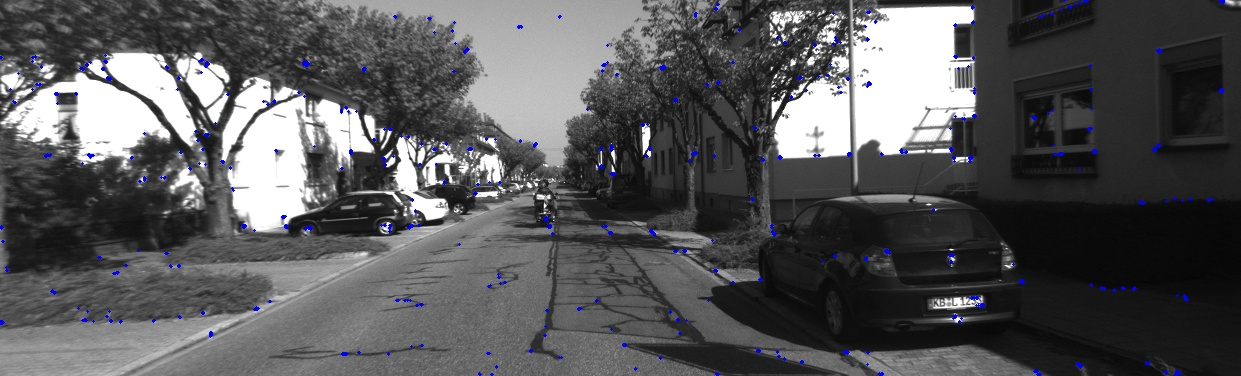
\includegraphics[width=0.8\textwidth]{corners1}
    \caption{Binned Harris corners overlaid on image 1}
    \label{fig:corner_image1}
    \end{subfigure}
    \begin{subfigure}[b]{\textwidth}
    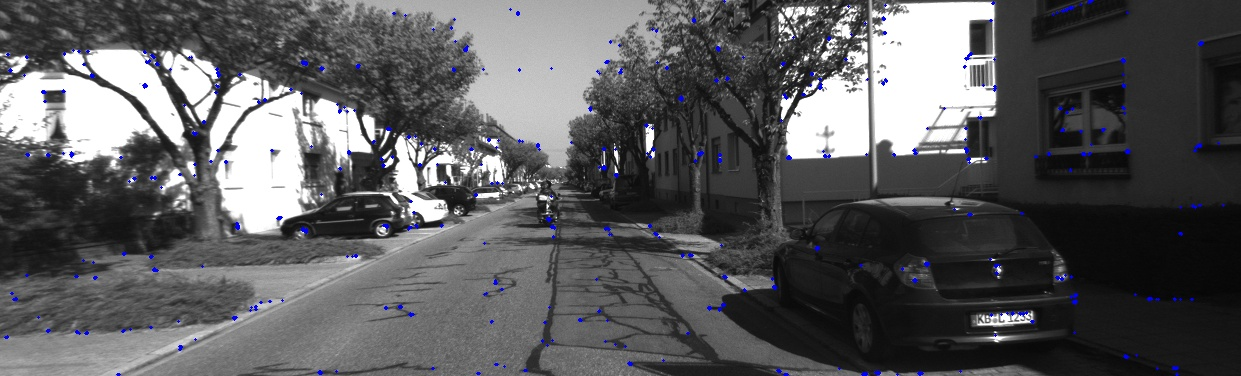
\includegraphics[width=0.8\textwidth]{corners2}
    \caption{Binned Harris Corners overlaid on image 2}
    \label{fig:corner_image1}
    \end{subfigure}
    \caption{The output of the Binned Harris corner detector overlaid on 3 subsequent images taken by the left camera of the KITTI data set.  The algorithm tracks these corners between each subsequent pair of images. The track is only one step long, in each new image the features are detected again and (independently of the previous tracks) are tracked into the following image}
\end{figure}

As a feature point descriptor we use a square patch of constant size. We experimentally chose a descriptor window size (11 pixels).

It should be said that there are a lot of feature point detectors/descriptors out there at the moment.  We chose Harris because it is quick, shows good performance in feature tracking in urban frame sequences and and may be easily implemented.

\subsection{Feature Matching}
There are two scenarios in which features are matched in the algorithm.

\begin{enumerate}
\item First matching is basically a feature tracking procedure.  For each feature found in previous image we look for a closest match in a new image.  We start a search in the same location where the feature was found in previous image and assume that image motion was not too large (this is a common assumption for video sequences).  We also assume that the feature patch did not change much and the metric that is used is SSD.  This is motivated by works like \cite{Shi94goodfeatures} (they also use patch deformation estimation to decide if the tracker has lost a track of the patch, which we currently do not do, but we may implement this in the future).
\item Another time, the features are matched across the images of the stereo-pair.  This matching procedure is relatively ``simple'' because the search for a match is limited only to a corresponding epipolar line. So when matching the features of the stereo pair, we search only along a horizontal scan-line, since the images are assumed to be rectified. Example matching is shown in ~\ref{fig:stereo_match}
\end{enumerate}

SSD-based procedure described above is prone to outliers. The algorithm implements additional heuristic procedure, called circular match, to deal with this issue.  Circular match treats a feature as matched in current stereo pair only if it matched successfully in between the stereo views and its tracks into previous stereo pair images matched as well.  This heuristics is effectively filtering out a large percentage of outlier matches, though not all of them. A typical image of a circular match output is presented in figure ~\ref{fig:circle}
\begin{figure}[h]
    \centering
    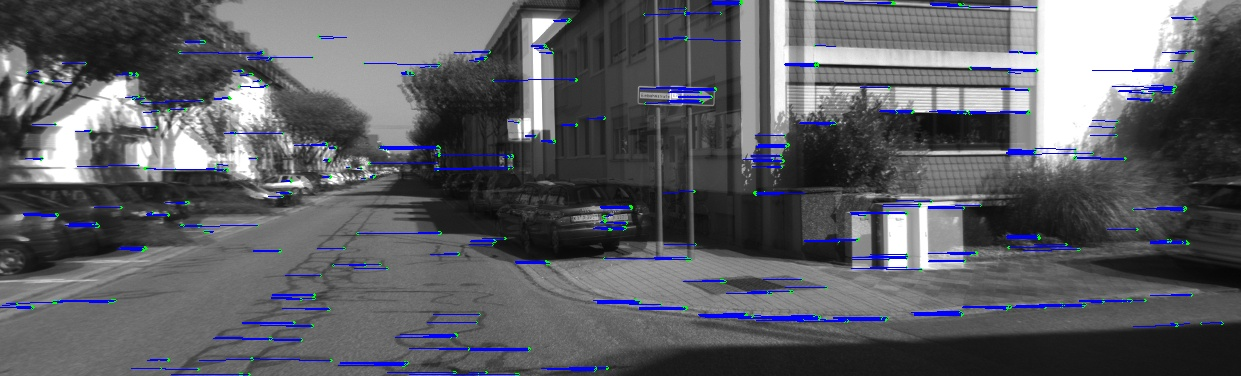
\includegraphics[width=0.8\textwidth]{blend}
    \caption{Images of the left and the right cameras are blended together to produce a single image.  Feature points are overlaid over a corresponding image and the match is shown by a blue line.}
    \label{fig:stereo_match}
\end{figure}

\begin{figure}[h]
    \centering
    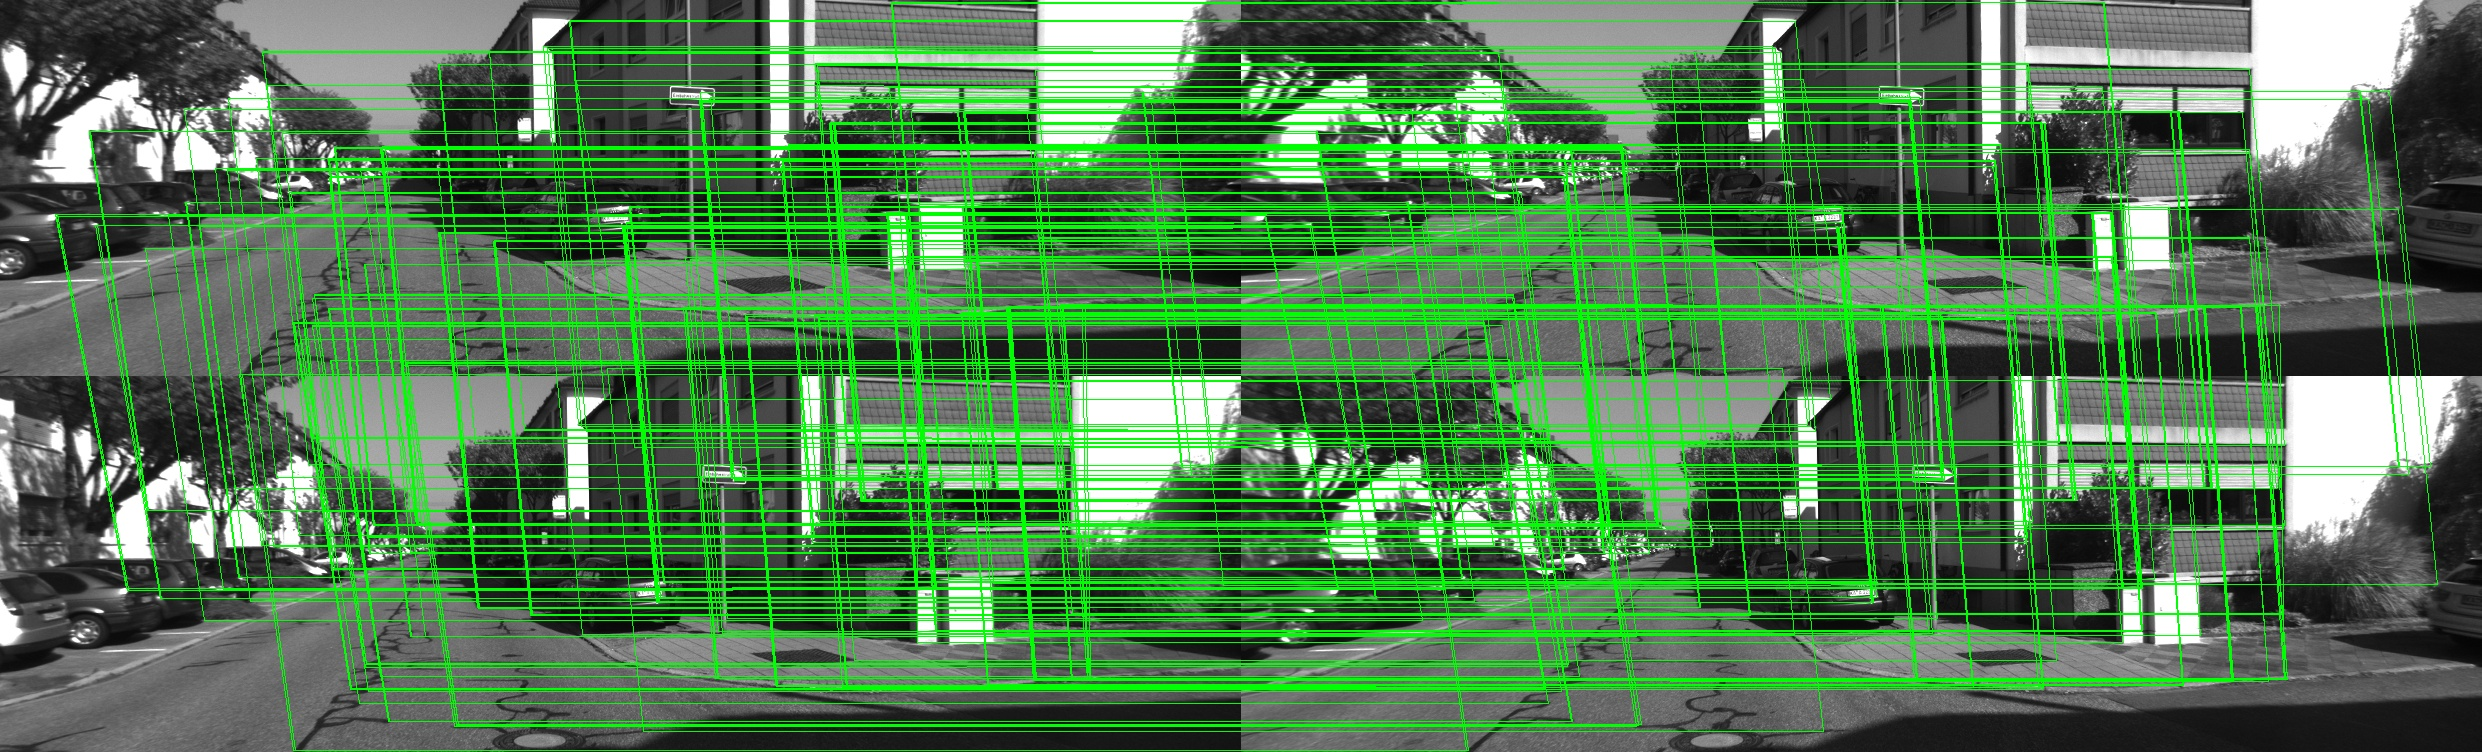
\includegraphics[width=0.8\textwidth]{circles}
    \caption{Example of circular match output. Left (right) columns show subsequent images of a left (right) camera respectively.  The match is considered successful only if it is consistent both in previous and current stereo pairs.}
    \label{fig:circle}
\end{figure}

\subsection{Parameter estimation procedure}

At the beginning of this step we have a set of features that their locations are known in images of both current and previous stereo pair.  Our goal is to estimate the motion of the camera between the poses at which these images were taken.  

The paragraphs below have some amount of notations and formulas, while basically we would like to carry out a simple procedure:\emph{Use camera calibration to find 3d locations of a features from previous stereo pair and use Gauss-Newton optimization to search for such camera motion parameter vector $x=\textbf{[r,t]}=(r_x,r_y,r_z,t_x,t_y,t_z)$ that minimizes image plane re-projection error in the current stereo pair}

Usually it takes a small number of iterations for the algorithm to converge.  Since there is still and option that circular match produces outliers, the whole optimization procedure is wrapped into RANSAC step.  During each RANSAC iteration we use a small number (3) of points to estimate the motion of the camera and return as an answer a set of parameters that are produced by the largest support set of all RANSAC iterations.

\subsubsection{Notation}
\begin{enumerate}

\item We use the following notation in the subsequent paragraphs: \begin{align*}
&cos(r_x)=c_x&sin(r_x)=s_x\\
&cos(r_y)=c_y&sin(r_y)=s_y\\
&cos(r_z)=c_z&sin(r_z)=s_z\\
\end{align*}

\item Let $X_i\in R^3,i=1...N$ be the coordinates of a 3d point as seen in the coordinate frame of previous camera position

\item Let $\textbf{r,t}\in R^3$ be the vectors describing the rotation and translation of the camera, s.t. $[\textbf{R(r),t}]*X_i$ describes the same 3d point in the coordinate frame of current camera position.

\item Camera intrinsics are $K=\left( \begin{array}{ccc} f& 0& c_u\\ 0& f& c_v\\0& 0& 1\\ \end{array}\right)$

\item Rotation matrix parameterized by Euler angles: $R(r) = R_x(r_x)R_y(r_y)R_z(r_z)$
\begin{align*}
R(r) &= \begin{pmatrix}
c_yc_z& -c_ys_z& s_y\\
c_xs_z+c_zs_xs_y& c_xc_z-s_xs_ys_z& -c_ys_x\\
s_xs_z-c_xc_zs_y& c_zs_x+c_xs_ys_z& c_xc_y
\end{pmatrix}
\end{align*}
Derivatives of the rotation matrix may be obtained in a straighforward manner, for example:
\begin{align*}
\frac{\partial R(r)}{\partial r_x} &= \begin{pmatrix}
0& 0& 0\\
-s_xs_z+c_zc_xs_y& -s_xc_z-c_xs_ys_z& -c_yc_x\\
s_xs_z+s_xc_zs_y& c_zc_x-s_xs_ys_z& -s_xc_y
\end{pmatrix}
\end{align*}
\item Let left/right camera projections of a rotated 3d point be $\pi^{(l)}$ and $\pi^{(r)}$ respectively, we may refer to these as to predicted locations of features
\begin{align*}
\pi_i^{(l)}(\textbf{r,t};X_i) &= K*[\textbf{R(r),t}]*X_i\\
\pi_i^{(r)}(\textbf{r,t};X_i) &= K*([\textbf{R(r),t}]*X_i - [base,0,0]^T)
\end{align*}
Derivation of the projections (right camera projection is obtained in a similar way):
\begin{align*}
\frac{\partial \pi_i^{(l)}(x)}{\partial x_j} &= \frac{\partial }{\partial x_j}\Bigg[K*[\textbf{R(r),t}]*X_i\Bigg]
\end{align*}
\item Observed locations of feature points in the current frame are given by $x_i^{(l)}$ and $x_i^{(r)}$
\item Image plane residuals (current frame) for feature point $i$ are given by:
\begin{align*}
r_i^{(l)}(\textbf{r,t}) &= \norm{x_i^{(l)}-\pi_i^{(l)}(\textbf{r,t};X_i)}\\
r_i^{(r)}(\textbf{r,t}) &= \norm{x_i^{(r)}-\pi_i^{(r)}(\textbf{r,t};X_i)}
\end{align*}
\item Let us define the following objective:
\begin{align*}\label{eq:objective}
f(\textbf{r,t}) =\sum_i^N[r_i^{(l)}[\textbf{r,t})]^2+\sum_i^N[r_i^{(r)}(\textbf{r,t})]^2
\end{align*}
Rewriting the above element wise:
\begin{align*}
f(\textbf{r,t})&=\sum_i^N\Bigg[\Big(x_i^{(l)}[0]-\frac{\pi_i^{(l)}[0]}{\pi_i^{(l)}[2]}\Big)^2+\Big(x_i^{(l)}[1]-\frac{\pi_i^{(l)}[1]}{\pi_i^{(l)}[2]}\Big)^2\\
&+\Big(x_i^{(r)}[0]-\frac{\pi_i^{(r)}[0]}{\pi_i^{(r)}[2]}\Big)^2+\Big(x_i^{(r)}[1]-\frac{\pi_i^{(r)}[1]}{\pi_i^{(r)}[2]}\Big)^2\Bigg]\\
\end{align*}


Note that the division is to convert homogeneous coordinates to pixel coordinates.

Now we define pixel coordinate residuals:
\[
r_j(x)= 
\begin{dcases}
  x_i^{(l)}[0]-\frac{\pi_i^{(l)}[0]}{\pi_i^{(l)}[2]},&  j = 4i+0, i=1..N\\
  x_i^{(l)}[1]-\frac{\pi_i^{(l)}[1]}{\pi_i^{(l)}[2]},&  j = 4i+1, i=1..N\\
  x_i^{(r)}[0]-\frac{\pi_i^{(r)}[0]}{\pi_i^{(r)}[2]},&  j = 4i+2, i=1..N\\
  x_i^{(r)}[1]-\frac{\pi_i^{(r)}[1]}{\pi_i^{(r)}[2]},&  j = 4i+3, i=1..N
\end{dcases}
\]

Finally, the objective may be expressed as:
\begin{align*}
f(\textbf{r,t})&=\sum_j^{4N} r_j^2\textbf{(r,t)}
\end{align*}
Odometry is posed as a minimization problem:
\begin{equation*}
\begin{aligned}
\textbf{[r,t]} = \underset{\textbf{r,t}}{\text{argmin}} f(\textbf{r,t})\\
\end{aligned}
\end{equation*}

\end{enumerate}

\subsubsection{Optimization Details}
\label{sec: optimization}
Let $r(x) = (r_1(x),r_2(x),r_3(x)...),i=1...4N$, then $f(x) = \frac{1}{2}\norm{r(x)}^2$.  The derivatives of $f(x)$ may be expressed in terms of the Jacobian of $r$:
$$
J(x) = \begin{bmatrix}\frac{\partial r_i}{\partial x_j} \end{bmatrix}_{i=1..N,j=1..6}
$$
We have:
\begin{align*}
\nabla f(x) &= \sum_{j=1}^{N}r_j(x)\nabla r_j(x)=J(x)^Tr(x)\\
\nabla^2 f(x) &= \sum_{j=1}^N\nabla r_j(x)\nabla r_j(x)^T+\sum_{j=1}^{N}r_j(x)\nabla^2 r_j(x)\\
&= J(x)^TJ(x) + \sum_{j=1}^{N}r_j(x)\nabla^2 r_j(x) \approx  J(x)^TJ(x)
\end{align*}

When the last equation is a Gauss-Newton approximation of the Hessian matrix.

Taking the derivatives of the residuals (other three are computed similarly):

$$
  \frac{\partial r_{4i}}{\partial x_j} = \Bigg[\frac{\partial \pi_i^{(l)}[0]}{\partial x_j}\pi_i^{(l)}[2]-\frac{\partial \pi_i^{(l)}[2]}{\partial x_j}\pi_i^{(l)}[0]\Bigg]\Big(\pi_i^{(l)}[2]\Big)^{-2}
$$

Gauss-Newton search direction is found by solving the following equation:
$$
J_k^TJ_kp_k^{GN}=-J_k^Tr_k
$$
\section{Results}

We use the KITTI data set \cite{Geiger2012CVPR} to evaluate our algorithm. VO algorithms are evaluated in terms of relative rotation/translation error that they produce over a number of image sequences taken primarily in urban environment.  Note that the algorithm is currently evaluated only for one of the sequences of the data set (00). 

As graphs in figure ~\ref{fig:results} state our algorithm produces about 0.016 deg/m and about 6\% of rotation and translation error respectively, which places us at about between places 28 and 29 in the ledger of competing algorithms over the KITTI data set (out of 32).

\begin{figure}[h]
    \centering
    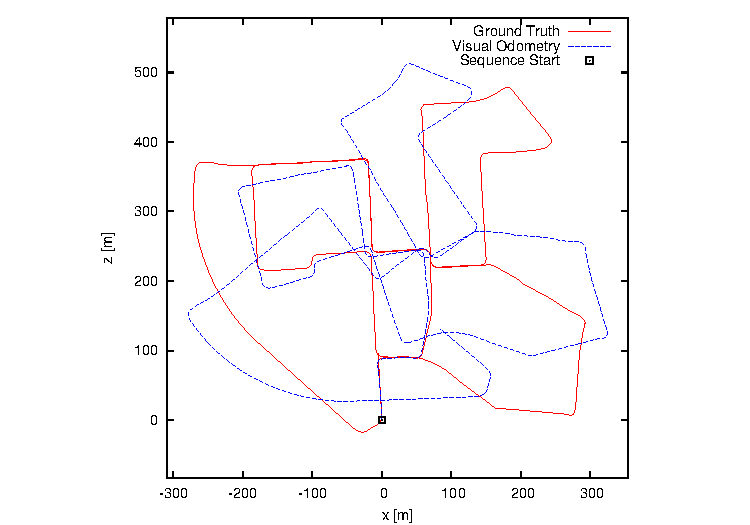
\includegraphics[width=0.8\textwidth]{00}
    \caption{Red line is the ground truth path while glue dotted line is the output of our algorithm.  Note that the errors of separate steps are accumulating throughout the whole sequence.}
    \label{fig:stereo_match}
\end{figure}

\begin{figure}[h]
    \centering
    \begin{subfigure}[b]{.49\textwidth}
    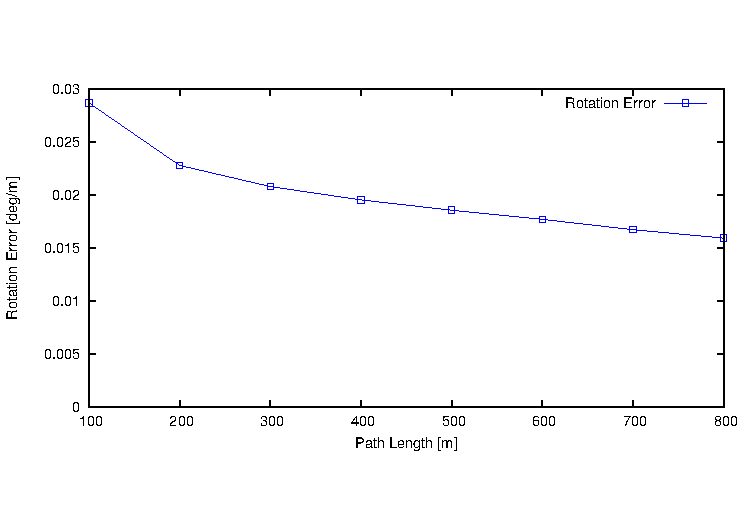
\includegraphics[width=1\textwidth]{00_rl}
    \caption{Rotation error vs. path length}
    \label{fig:rotation_error}
    \end{subfigure}
    \begin{subfigure}[b]{.49\textwidth}
    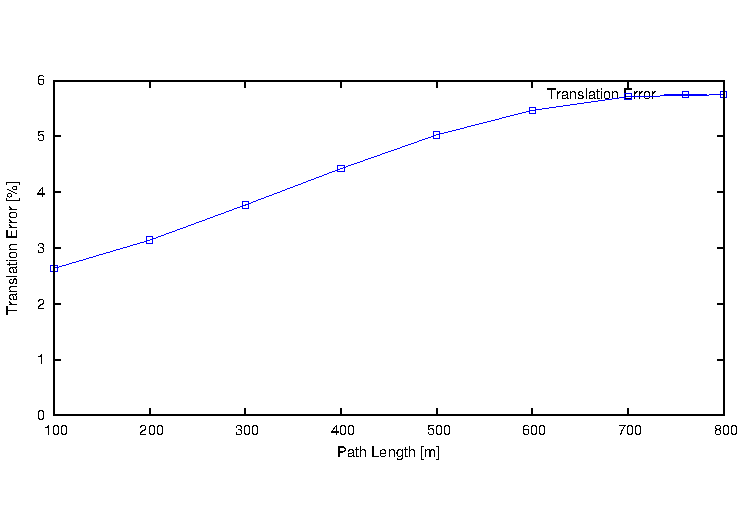
\includegraphics[width=1\textwidth]{00_tl}
    \caption{Translation error vs. path length.}
    \label{fig:translation_error}
    \end{subfigure}
    \caption{The algorithm produces about 0.016 deg/m and about 6\% of rotation and translation error respectively, which places us at about between places 28 and 29 in the ledger of competing algorithms over the KITTI data set}
    \label{fig:results}
\end{figure}

\section{Discussion and future work}

\subsection{Statistical VO}

The idea is to improve VO by incorporating statistical information about the features and the triangulation into parameter estimation process. Some of the details needs to be worked on, but the the overall plan of action may be as follows:
\begin{enumerate}
  
\item Estimate uncertainty (i.e. a covariance matrix) of each corner. There are a number of ways to measure the uncertainty for Harris corners, (e.g., \cite{orguner2007statistical}).  The result is a pair of covariance matrices $\Sigma_L,\Sigma_R$ for left/right corner respectively.
\item Estimate uncertainty of the 3d point $X$. Using the $\Sigma_L,\Sigma_R$  we may estimate the uncertainty of the triangulated 3d point using a method proposed in \cite{matthies1989dynamic} (this is commonly reffered to as ``sandwitch covariance''):
\[
\Sigma_{X} = J diag(\Sigma_L, \Sigma_R) J'
\]
Here J is the Jacobian of the triangulation procedure (it may either be calculated analytically or computed numerically, depending on the triangulation algorithm).
\item Using ``sandwitch covariance'' once again compute the covariances of the predicted corners.
\item Incorporate the image plane uncertainty into the reprojection minimization process.
\[
\textbf{[r,t]} = \underset{\textbf{r,t}}{\text{argmin}} \sum_i (x_i-\hat{x}_i(\textbf{r,t}))'\Sigma_{x_i}(\textbf{r,t})(x_i-\hat{x}_i(\textbf{r,t}))
\]
where $x,\hat{x}$ are observed and predicted feature locations, and $\textbf{r,t}$ are camera motion parameters.
\end{enumerate}
\subsection{Detect relative motions in the scene}

Some uses of VO are in urban scenes.  There is a lot of motion (e.g., cars, buses, pedestrians, etc.).  I don't have a solution here, but it may be nice if the algorithm could somehow disregard the features that belongs to such moving objects.

\section{Appendices}
\subsection{Rotation matrices}
\label{sec: rotation matrices}
\begin{align*}
R_x(r_x) &= 
\begin{pmatrix}
1& 0& 0\\
0& c(r_x)& -s(r_x)\\
0& s(r_x)& c(r_x)
\end{pmatrix} &\frac{\partial R_x}{\partial r_x} = \begin{pmatrix}
0& 0& 0\\
0& -s(r_x)& -c(r_x)\\
0& c(r_x)& -s(r_x)
\end{pmatrix}\\
R_y(r_y) &= \begin{pmatrix}
c(r_y)& 0& s(r_y)\\
0& 1& 0\\
-s(r_y)& 0& c(r_y)
\end{pmatrix} &\frac{\partial R_y}{\partial r_y} = \begin{pmatrix}
-s(r_y)& 0& c(r_y)\\
0& 0& 0\\
-c(r_y)& 0& -s(r_y)
\end{pmatrix}\\
R_z(r_z) &= \begin{pmatrix}
c(r_z)& -s(r_z)& 0\\
s(r_z)& c(r_z)& 0)\\
0& 0& 1
\end{pmatrix} &\frac{\partial R_y}{\partial r_y} = \begin{pmatrix}
-s(r_z)& -c(r_z)& 0\\
c(r_z)& -s(r_z)& 0)\\
0& 0& 1
\end{pmatrix}
\end{align*}

\subsection{Derivative of camera projection}
\begin{align*}
\frac{\partial \pi^{(l)}}{\partial r_x} &= K*\frac{\partial }{\partial r_x}\Big[R(r),t\Big]*X_i\\
&= \begin{pmatrix} f& 0& c_u\\ 0& f& c_v\\0& 0& 1\\ \end{pmatrix}\begin{pmatrix}
0& 0& 0& 0\\
-s_xs_z+c_zc_xs_y& -s_xc_z-c_xs_ys_z& -c_yc_x&0\\
s_xs_z+s_xc_zs_y& c_zc_x-s_xs_ys_z& -s_xc_y&0
\end{pmatrix}\begin{pmatrix}X\\Y\\Z\\1\end{pmatrix}\\
&=\begin{pmatrix} f& 0& c_u\\ 0& f& c_v\\0& 0& 1\\ \end{pmatrix}\begin{pmatrix}
0\\
X(-s_xs_z+c_zc_xs_y)-Y(s_xc_z+c_xs_ys_z)-Zc_yc_x\\
X(s_xs_z+s_xc_zs_y)+Y(c_zc_x-s_xs_ys_z)-Zs_xc_y
\end{pmatrix}\\
\end{align*}

\bibliographystyle{plain}
\bibliography{simple}
\end{document}

